\subsection{Ricerca} \label{Ricerca}
Un problema fondamentale dei siti è far sì che il proprio contenuto sia trovato dagli utenti. La ricerca diviene quindi un fattore fondamentale all'interno del web. Ogni sito internet, se abbastanza grande, dovrebbe avere come servizio la ricerca interna. In questo caso il sito presenta una dimensione  contenutistica molto elevato quindi la modalità di ricerca è essenziale.
\nomeSito\ ha optato per la ricerca classica nella quale si inseriscono una serie di parole chiave e si preme il pulsante "Cerca" che manda in esecuzione la ricerca di tutti i contenuti collegati a quella parola.
Il problema è che tale tipo di ricerca lo si ritrova unicamente nella homepage. Le altre pagine non presentano questo strumento assai utile. Il box permette di inserire 26 caratteri visibili, ma ne accetta infiniti. Inoltre, è molto limitata perché costringe un utente a sapere cosa cercare e quindi deve andare in altri siti per decidere cosa guardare. La soluzione migliore sarebbe quella di categorizzare gli anime in base a dei tag. Una modalità simile viene adottata a fondo pagina ma risulta scomoda così come è stata ideata (bloated-design). Sarebbe meglio togliere l'effetto grafico che è stato inserito e migliorare la modalità di ricerca statica.

\paragraph{Caso limite}
Spesso può capitare di imbattersi in una ricerca che non fornisce alcun risultato. Quando ciò accade l'utente si aspetta di ottenere un messaggio che gli comunichi l'accaduto. Tuttavia una buona cosa è dare la possibilità all'utente di navigare nuovamente nel sito e fornirgli dei suggerimenti, portandolo a guardare qualcosa di simile a quello che stava cercando o analizzando le ultime uscite. L'immagine che segue riporta una ricerca con 0 risultati. Non vi è alcun consiglio, l'unica informazione è  la frase "Nothing to see here.". 

\begin{figure}[H]
	\centering
	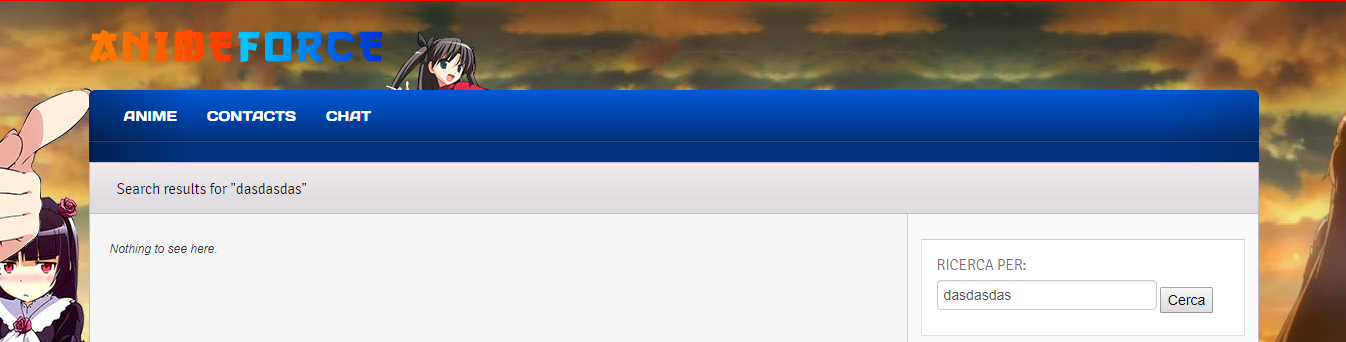
\includegraphics[width=1\textwidth]{img/CasoLimite.png}
	\caption{Caso limite} 
	\label{img5} 
\end{figure}
